% se define una variable condicional para cada formato de salida
\newif\ifPDF%
\newif\ifBLACKPDF%
\newif\ifEPUB%
\newif\ifHTML%
\newif\ifODT%

%\PDFtrue
%\BLACKPDFtrue
%\EPUBtrue
\HTMLtrue
%\ODTtrue

% agregamos las referencias
\addbibresource{./files/gbTeXbib-CHARLAUNPaz.bib}
% agregamos el glosario

\newglossaryentry{@glo203-unpaz}{
type = \acronymtype,
name         = {UNPAZ},
first        = {Universidad Nacional de José C. Paz (UNPAZ)},
text         = {UNPAZ},
}
\newglossaryentry{@glo204-libro}{
name         = {libro},
description  = {(del latín \emph{liber, libri}) es una obra impresa, manuscrita o pintada en una serie de hojas de papel, pergamino, vitela u otro material, unidas por un lado (es decir, encuadernadas) y protegidas con tapas, también llamadas cubiertas. Un libro puede tratar sobre cualquier tema. Según la definición de la Unesco,​ un libro debe poseer al menos veinticinco hojas (49 páginas), pues de veinticuatro hojas o menos sería un folleto; y de una hasta cuatro páginas se consideran hojas sueltas (en una o dos hojas)},
first        = {libro},
text         = {libro},
}

\ifPDF
\usepackage[hyphenation,homeoarchy,draft,homeoarchywordcolor=yellow,homeoarchycharcolor=orange]{impnattypo}
\usepackage[allcolors=magenta,colorlinks]{hyperref}
\boolfalse{FileSectionNames}
\renewcommand{\linkhomename}{Inicio}
\renewcommand{\linkpreviousname}{Anterior}
\renewcommand{\linknextname}{Siguiente}
\renewcommand{\sidetocname}{Sumario}
\setcounter{tocdepth}{1}
\setcounter{secnumdepth}{2}
\setcounter{FileDepth}{1}
\setcounter{FootnoteDepth}{1}
\booltrue{CombineHigherDepths}
\setcounter{SideTOCDepth}{1}
\CSSFilename{imago_custom.css}
\HTMLPageBottom{\LinkPrevious | \LinkNext}
\HTMLFirstPageTop{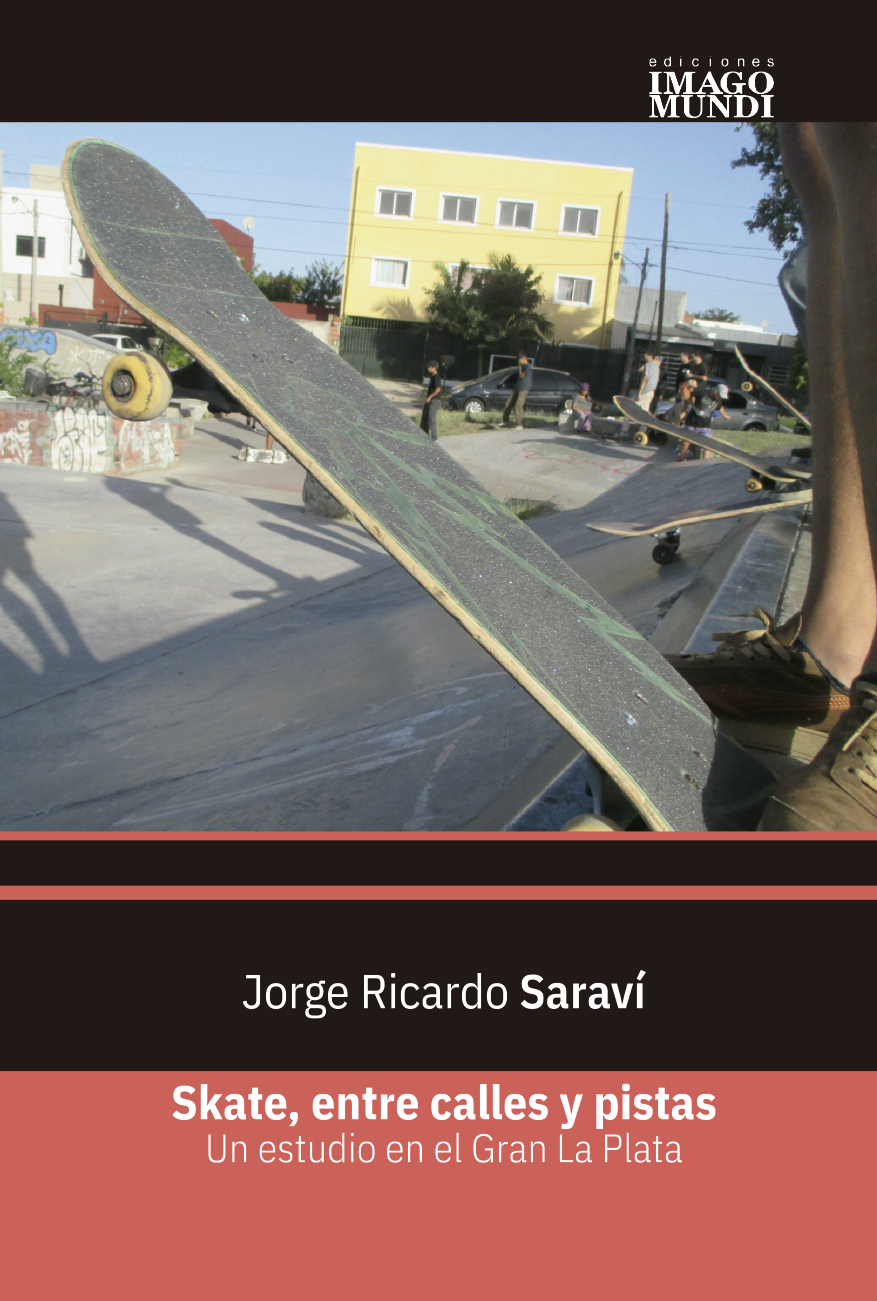
\includegraphics[width=5cm]{./media/cover.png}}
\HTMLTitle{Literatura y Pensamiento}
\HTMLLanguage{es-ES}
\HTMLAddMeta{DC.language}{es-ES}
\HTMLAuthor{Andrés Racket}
\HTMLAddMeta{DC.creator}{Andrés Racket}
\HTMLFirstPageBottom{
\includegraphics[width=30mm]{./media/unpaz_logo.png}}
\HTMLAddMeta{isbn}{978-987-8262-33-8}
\HTMLAddMeta{book-title}{Literatura y Pensamiento}
\HTMLAddMeta{twitter:title}{Literatura y Pensamiento}
\HTMLAddMeta{DC.title}{Literatura y Pensamiento}
\HTMLAddMeta{subtitle}{Caja de herramientas para el análisis literario}
\HTMLAddMeta{volume}{1}
\HTMLAddMeta{edition}{Primera}
\HTMLAddMeta{license}{CC BY-NC 4.0 Attribution-NonCommercial 4.0 International}
\HTMLAddMeta{DC.rights}{CC BY-NC 4.0 Attribution-NonCommercial 4.0 International}
\HTMLAddMeta{keywords}{clave1,clave2,clave3,clave4}
\HTMLAddMeta{DC.subject}{clave1,clave2,clave3,clave4}
\HTMLAddMeta{series}{Ciencias Sociales}
\HTMLAddMeta{language}{es}
\HTMLAddMeta{page-count}{224}
\HTMLAddMeta{dimensions}{14x20cm}
\HTMLAddMeta{illustrator}{Nombre y Apellido del ilustrador}
\HTMLAddMeta{translator}{Nombre y Apellido del traductor}
\HTMLAddMeta{genre}{Ciencias Sociales}
\HTMLAddMeta{description}{Resumen en idioma principal}
\HTMLAddMeta{twitter:description}{Resumen en idioma principal}
\HTMLAddMeta{format}{book}
\HTMLAddMeta{editor}{Desconocida}
\HTMLAddMeta{publication-date}{2023/12/01}
\HTMLAddMeta{DC.date}{2023/12/01}
\HTMLAddMeta{annotation}{Acá van comentarios sobre el libro}
\HTMLAddMeta{audience}{Estudiantes universitarios}
\HTMLAddMeta{DC.audience}{Estudiantes universitarios}
\HTMLAddMeta{binding}{Encolado}
\HTMLAddMeta{DC.isPartOf}{Morral de apuntes}
\HTMLAddMeta{DC.source}{CHARLAUNPaz.tex}
\HTMLAddMeta{DC.identifier}{https://edunpaz.unpaz.edu.ar/OMP/index.php/edunpaz/catalog/book/108}

\usepackage{hyperxmp}
	\else
	\ifBLACKPDF
	\usepackage[cam,width=18truecm,height=25.5truecm,center]{crop}
	\usepackage[draft]{hyperref}
	\boolfalse{FileSectionNames}
\renewcommand{\linkhomename}{Inicio}
\renewcommand{\linkpreviousname}{Anterior}
\renewcommand{\linknextname}{Siguiente}
\renewcommand{\sidetocname}{Sumario}
\setcounter{tocdepth}{1}
\setcounter{secnumdepth}{2}
\setcounter{FileDepth}{1}
\setcounter{FootnoteDepth}{1}
\booltrue{CombineHigherDepths}
\setcounter{SideTOCDepth}{1}
\CSSFilename{imago_custom.css}
\HTMLPageBottom{\LinkPrevious | \LinkNext}
\HTMLFirstPageTop{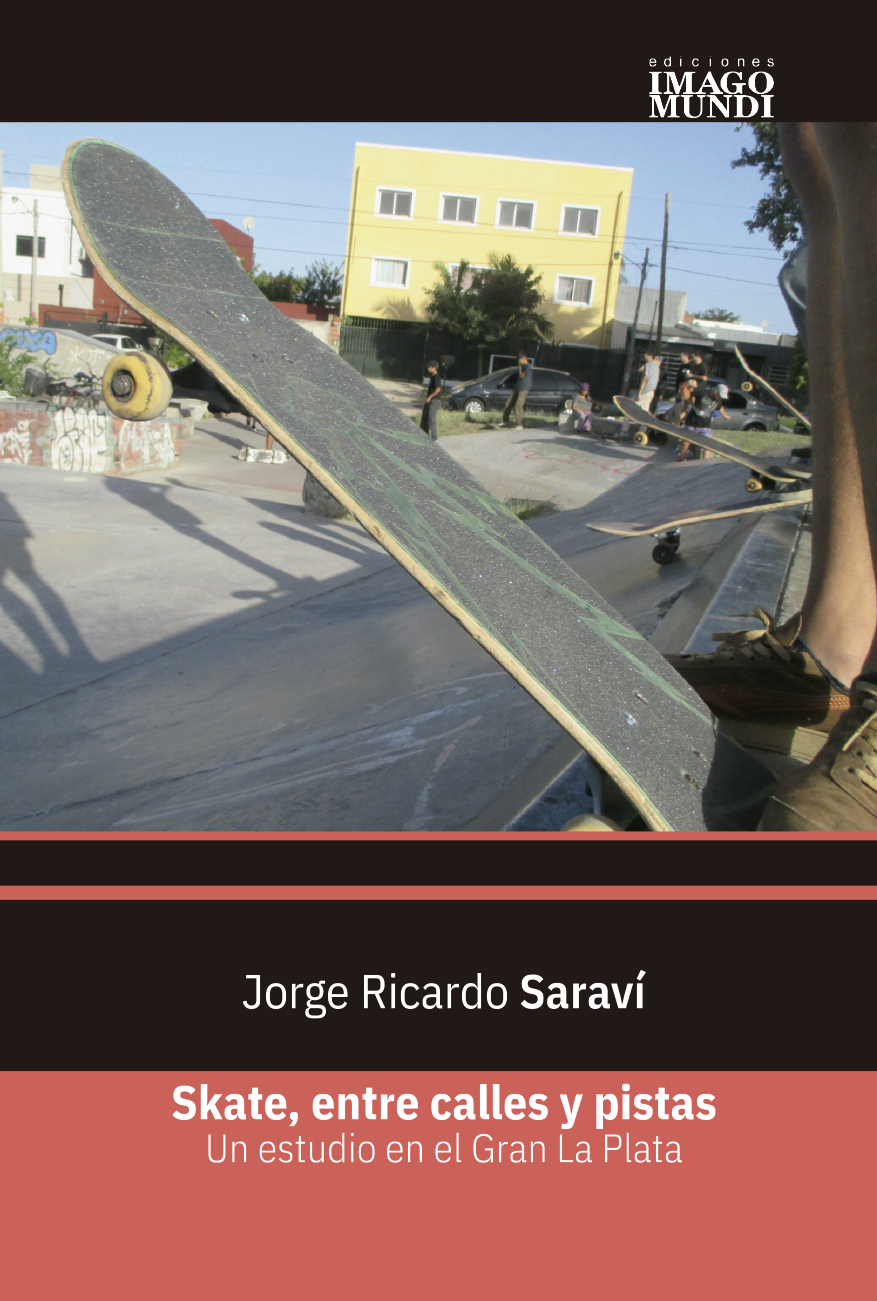
\includegraphics[width=5cm]{./media/cover.png}}
\HTMLTitle{Literatura y Pensamiento}
\HTMLLanguage{es-ES}
\HTMLAddMeta{DC.language}{es-ES}
\HTMLAuthor{Andrés Racket}
\HTMLAddMeta{DC.creator}{Andrés Racket}
\HTMLFirstPageBottom{
\includegraphics[width=30mm]{./media/unpaz_logo.png}}
\HTMLAddMeta{isbn}{978-987-8262-33-8}
\HTMLAddMeta{book-title}{Literatura y Pensamiento}
\HTMLAddMeta{twitter:title}{Literatura y Pensamiento}
\HTMLAddMeta{DC.title}{Literatura y Pensamiento}
\HTMLAddMeta{subtitle}{Caja de herramientas para el análisis literario}
\HTMLAddMeta{volume}{1}
\HTMLAddMeta{edition}{Primera}
\HTMLAddMeta{license}{CC BY-NC 4.0 Attribution-NonCommercial 4.0 International}
\HTMLAddMeta{DC.rights}{CC BY-NC 4.0 Attribution-NonCommercial 4.0 International}
\HTMLAddMeta{keywords}{clave1,clave2,clave3,clave4}
\HTMLAddMeta{DC.subject}{clave1,clave2,clave3,clave4}
\HTMLAddMeta{series}{Ciencias Sociales}
\HTMLAddMeta{language}{es}
\HTMLAddMeta{page-count}{224}
\HTMLAddMeta{dimensions}{14x20cm}
\HTMLAddMeta{illustrator}{Nombre y Apellido del ilustrador}
\HTMLAddMeta{translator}{Nombre y Apellido del traductor}
\HTMLAddMeta{genre}{Ciencias Sociales}
\HTMLAddMeta{description}{Resumen en idioma principal}
\HTMLAddMeta{twitter:description}{Resumen en idioma principal}
\HTMLAddMeta{format}{book}
\HTMLAddMeta{editor}{Desconocida}
\HTMLAddMeta{publication-date}{2023/12/01}
\HTMLAddMeta{DC.date}{2023/12/01}
\HTMLAddMeta{annotation}{Acá van comentarios sobre el libro}
\HTMLAddMeta{audience}{Estudiantes universitarios}
\HTMLAddMeta{DC.audience}{Estudiantes universitarios}
\HTMLAddMeta{binding}{Encolado}
\HTMLAddMeta{DC.isPartOf}{Morral de apuntes}
\HTMLAddMeta{DC.source}{CHARLAUNPaz.tex}
\HTMLAddMeta{DC.identifier}{https://edunpaz.unpaz.edu.ar/OMP/index.php/edunpaz/catalog/book/108}

	\usepackage{hyperxmp}
		\else
		\ifEPUB

			\else
			\ifHTML
			\usepackage{hyperref}
			\boolfalse{FileSectionNames}
\renewcommand{\linkhomename}{Inicio}
\renewcommand{\linkpreviousname}{Anterior}
\renewcommand{\linknextname}{Siguiente}
\renewcommand{\sidetocname}{Sumario}
\setcounter{tocdepth}{1}
\setcounter{secnumdepth}{2}
\setcounter{FileDepth}{1}
\setcounter{FootnoteDepth}{1}
\booltrue{CombineHigherDepths}
\setcounter{SideTOCDepth}{1}
\CSSFilename{imago_custom.css}
\HTMLPageBottom{\LinkPrevious | \LinkNext}
\HTMLFirstPageTop{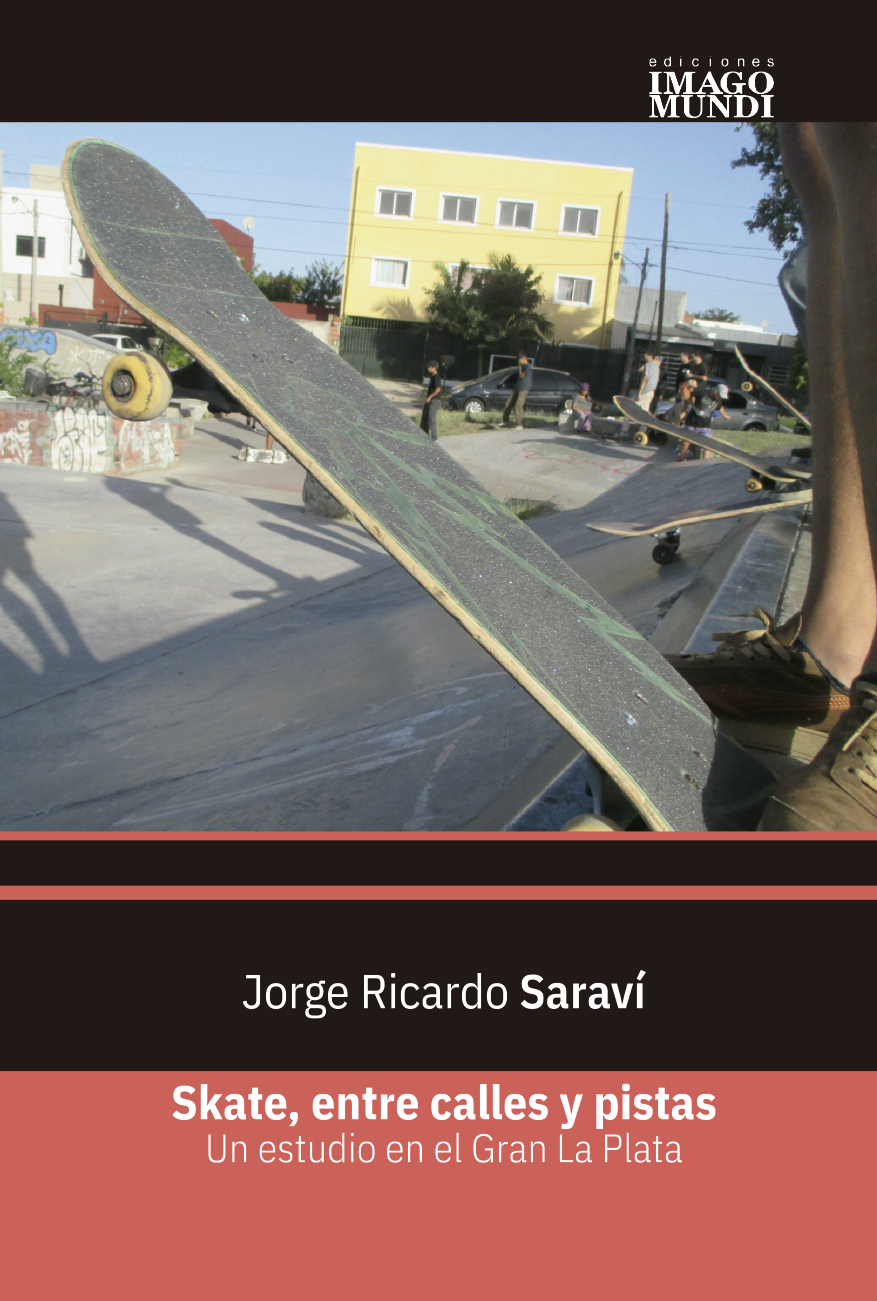
\includegraphics[width=5cm]{./media/cover.png}}
\HTMLTitle{Literatura y Pensamiento}
\HTMLLanguage{es-ES}
\HTMLAddMeta{DC.language}{es-ES}
\HTMLAuthor{Andrés Racket}
\HTMLAddMeta{DC.creator}{Andrés Racket}
\HTMLFirstPageBottom{
\includegraphics[width=30mm]{./media/unpaz_logo.png}}
\HTMLAddMeta{isbn}{978-987-8262-33-8}
\HTMLAddMeta{book-title}{Literatura y Pensamiento}
\HTMLAddMeta{twitter:title}{Literatura y Pensamiento}
\HTMLAddMeta{DC.title}{Literatura y Pensamiento}
\HTMLAddMeta{subtitle}{Caja de herramientas para el análisis literario}
\HTMLAddMeta{volume}{1}
\HTMLAddMeta{edition}{Primera}
\HTMLAddMeta{license}{CC BY-NC 4.0 Attribution-NonCommercial 4.0 International}
\HTMLAddMeta{DC.rights}{CC BY-NC 4.0 Attribution-NonCommercial 4.0 International}
\HTMLAddMeta{keywords}{clave1,clave2,clave3,clave4}
\HTMLAddMeta{DC.subject}{clave1,clave2,clave3,clave4}
\HTMLAddMeta{series}{Ciencias Sociales}
\HTMLAddMeta{language}{es}
\HTMLAddMeta{page-count}{224}
\HTMLAddMeta{dimensions}{14x20cm}
\HTMLAddMeta{illustrator}{Nombre y Apellido del ilustrador}
\HTMLAddMeta{translator}{Nombre y Apellido del traductor}
\HTMLAddMeta{genre}{Ciencias Sociales}
\HTMLAddMeta{description}{Resumen en idioma principal}
\HTMLAddMeta{twitter:description}{Resumen en idioma principal}
\HTMLAddMeta{format}{book}
\HTMLAddMeta{editor}{Desconocida}
\HTMLAddMeta{publication-date}{2023/12/01}
\HTMLAddMeta{DC.date}{2023/12/01}
\HTMLAddMeta{annotation}{Acá van comentarios sobre el libro}
\HTMLAddMeta{audience}{Estudiantes universitarios}
\HTMLAddMeta{DC.audience}{Estudiantes universitarios}
\HTMLAddMeta{binding}{Encolado}
\HTMLAddMeta{DC.isPartOf}{Morral de apuntes}
\HTMLAddMeta{DC.source}{CHARLAUNPaz.tex}
\HTMLAddMeta{DC.identifier}{https://edunpaz.unpaz.edu.ar/OMP/index.php/edunpaz/catalog/book/108}

			\title{Literatura y pensamiento}
			\date{\today}
				\else
				\ifODT
				\usepackage[unicode,hyperindex=true]{hyperref}
				\boolfalse{FileSectionNames}
\renewcommand{\linkhomename}{Inicio}
\renewcommand{\linkpreviousname}{Anterior}
\renewcommand{\linknextname}{Siguiente}
\renewcommand{\sidetocname}{Sumario}
\setcounter{tocdepth}{1}
\setcounter{secnumdepth}{2}
\setcounter{FileDepth}{1}
\setcounter{FootnoteDepth}{1}
\booltrue{CombineHigherDepths}
\setcounter{SideTOCDepth}{1}
\CSSFilename{imago_custom.css}
\HTMLPageBottom{\LinkPrevious | \LinkNext}
\HTMLFirstPageTop{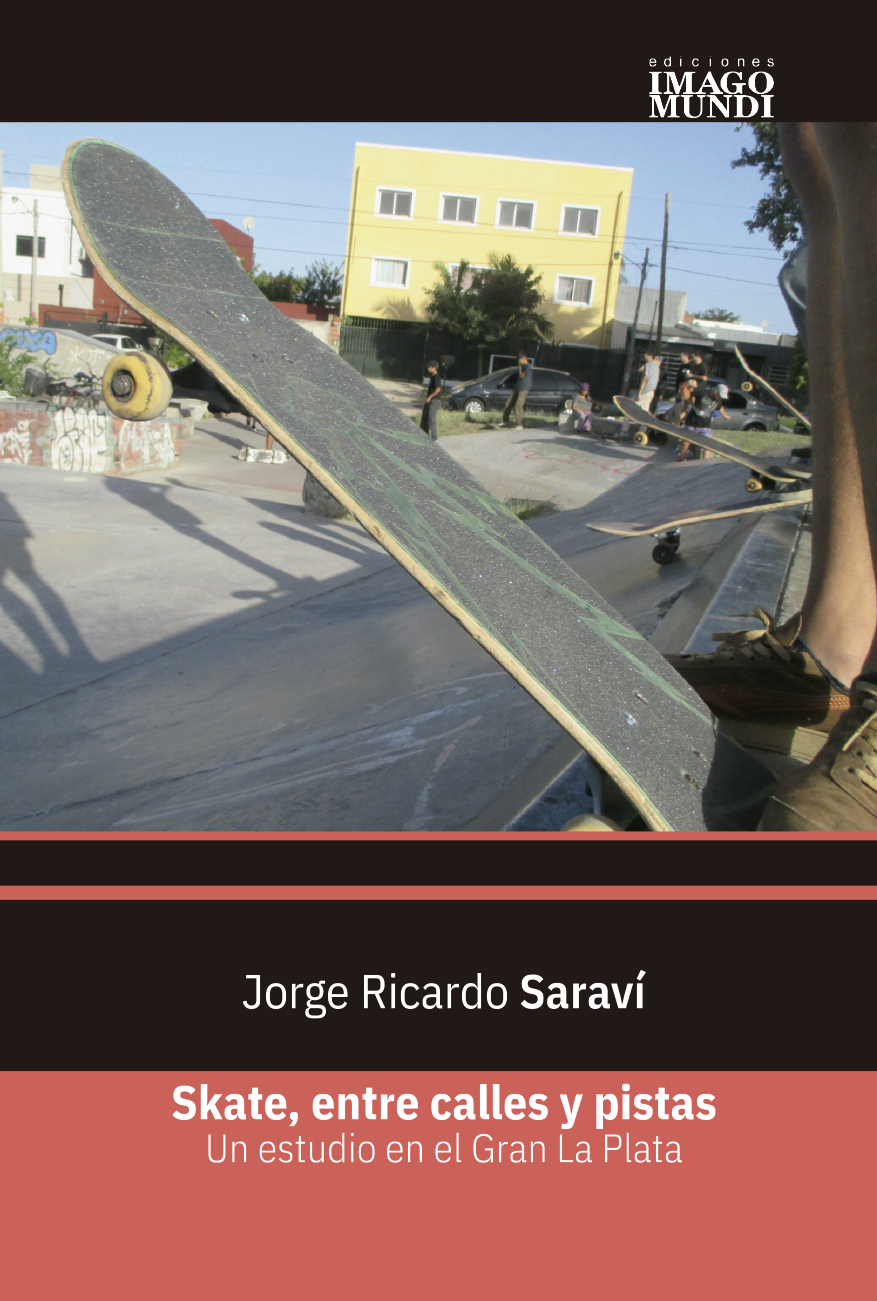
\includegraphics[width=5cm]{./media/cover.png}}
\HTMLTitle{Literatura y Pensamiento}
\HTMLLanguage{es-ES}
\HTMLAddMeta{DC.language}{es-ES}
\HTMLAuthor{Andrés Racket}
\HTMLAddMeta{DC.creator}{Andrés Racket}
\HTMLFirstPageBottom{
\includegraphics[width=30mm]{./media/unpaz_logo.png}}
\HTMLAddMeta{isbn}{978-987-8262-33-8}
\HTMLAddMeta{book-title}{Literatura y Pensamiento}
\HTMLAddMeta{twitter:title}{Literatura y Pensamiento}
\HTMLAddMeta{DC.title}{Literatura y Pensamiento}
\HTMLAddMeta{subtitle}{Caja de herramientas para el análisis literario}
\HTMLAddMeta{volume}{1}
\HTMLAddMeta{edition}{Primera}
\HTMLAddMeta{license}{CC BY-NC 4.0 Attribution-NonCommercial 4.0 International}
\HTMLAddMeta{DC.rights}{CC BY-NC 4.0 Attribution-NonCommercial 4.0 International}
\HTMLAddMeta{keywords}{clave1,clave2,clave3,clave4}
\HTMLAddMeta{DC.subject}{clave1,clave2,clave3,clave4}
\HTMLAddMeta{series}{Ciencias Sociales}
\HTMLAddMeta{language}{es}
\HTMLAddMeta{page-count}{224}
\HTMLAddMeta{dimensions}{14x20cm}
\HTMLAddMeta{illustrator}{Nombre y Apellido del ilustrador}
\HTMLAddMeta{translator}{Nombre y Apellido del traductor}
\HTMLAddMeta{genre}{Ciencias Sociales}
\HTMLAddMeta{description}{Resumen en idioma principal}
\HTMLAddMeta{twitter:description}{Resumen en idioma principal}
\HTMLAddMeta{format}{book}
\HTMLAddMeta{editor}{Desconocida}
\HTMLAddMeta{publication-date}{2023/12/01}
\HTMLAddMeta{DC.date}{2023/12/01}
\HTMLAddMeta{annotation}{Acá van comentarios sobre el libro}
\HTMLAddMeta{audience}{Estudiantes universitarios}
\HTMLAddMeta{DC.audience}{Estudiantes universitarios}
\HTMLAddMeta{binding}{Encolado}
\HTMLAddMeta{DC.isPartOf}{Morral de apuntes}
\HTMLAddMeta{DC.source}{CHARLAUNPaz.tex}
\HTMLAddMeta{DC.identifier}{https://edunpaz.unpaz.edu.ar/OMP/index.php/edunpaz/catalog/book/108}

				\fi
			\fi
		\fi
	\fi
\fi

\begin{document}
\frontmatter

\ifEPUB
	\ifdefined\HCode
	\phantomsection
	\addcontentsline{toc}{section}{Portada}
	\coverimage{./media/cover.png}
	\clearpage
	\fi
\fi

\ifPDF
% página 1
\newpage
\thispagestyle{empty}
{\textcolor{white}{.}}

% página 2
\newpage
\thispagestyle{empty}
{\textcolor{white}{.}}

% página 3
\newpage
\thispagestyle{empty}
{\textcolor{white}{.}}

\vspace{30mm}

\begin{center}
	\LARGE{<título>}
\end{center}

% página 4
\newpage
\thispagestyle{empty}
{\textcolor{white}{.}}

% página 5
\newpage
\thispagestyle{empty}
\begin{center}%,draft
{\sc\large{nombre de autor}}\\ %compiladoras
\end{center}

\vspace{30mm}

\begin{center}
\LARGE{título}\\\vspace{10mm}

\Large{subtítulo}
\end{center}

\vfill

\begin{figure}[b]
\centering

\includegraphics[width=30mm]{./media/unpaz_logo.png}
\end{figure}

% página 6
\newpage
\thispagestyle{empty}
\begin{figure}[t]
\centering
\vspace{-10mm}

\includegraphics[width=15mm]{./media/logo-GNU.png}\\
\sc{colección comunicación}
\end{figure}

\noindent autor \\
\noindent título. 1a ed. Buenos Aires: 2023.\\
\noindent 000 p.; 15.5x23 cm. ISBN 978-950-793-000-0 \\
\noindent 1. \\
\noindent CDD .\\
\noindent Fecha de catalogación: 00/00/20xx \\
\noindent \textcopyright~2024, autor \\
\noindent \textcopyright~2024, \\
\noindent Imagen de tapa: .\\
\noindent Hecho el depósito que marca la ley 11.723\\
\noindent Impreso en Argentina, tirada de esta edición: 000 ejemplares\\

\vfill

\noindent Ninguna parte de esta publicación, incluido el diseño de cubierta, puede ser reproducida, almacenada o transmitida de manera alguna ni por ningún medio, ya sea eléctrico, químico, mecánico, óptico, de grabación o de fotocopia, sin permiso previo por escrito del editor. Este libro se terminó de imprimir en el mes de xxxx de 20xx en San Carlos Impresiones, Virrey Liniers 2203, Ciudad Autónoma de Buenos Aires, República Argentina.

	\else
	\ifBLACKPDF
	% página 1
\newpage
\thispagestyle{empty}
{\textcolor{white}{.}}

% página 2
\newpage
\thispagestyle{empty}
{\textcolor{white}{.}}

% página 3
\newpage
\thispagestyle{empty}
{\textcolor{white}{.}}

\vspace{30mm}

\begin{center}
	\LARGE{<título>}
\end{center}

% página 4
\newpage
\thispagestyle{empty}
{\textcolor{white}{.}}

% página 5
\newpage
\thispagestyle{empty}
\begin{center}%,draft
{\sc\large{nombre de autor}}\\ %compiladoras
\end{center}

\vspace{30mm}

\begin{center}
\LARGE{título}\\\vspace{10mm}

\Large{subtítulo}
\end{center}

\vfill

\begin{figure}[b]
\centering

\includegraphics[width=30mm]{./media/unpaz_logo.png}
\end{figure}

% página 6
\newpage
\thispagestyle{empty}
\begin{figure}[t]
\centering
\vspace{-10mm}

\includegraphics[width=15mm]{./media/logo-GNU.png}\\
\sc{colección comunicación}
\end{figure}

\noindent autor \\
\noindent título. 1a ed. Buenos Aires: 2023.\\
\noindent 000 p.; 15.5x23 cm. ISBN 978-950-793-000-0 \\
\noindent 1. \\
\noindent CDD .\\
\noindent Fecha de catalogación: 00/00/20xx \\
\noindent \textcopyright~2024, autor \\
\noindent \textcopyright~2024, \\
\noindent Imagen de tapa: .\\
\noindent Hecho el depósito que marca la ley 11.723\\
\noindent Impreso en Argentina, tirada de esta edición: 000 ejemplares\\

\vfill

\noindent Ninguna parte de esta publicación, incluido el diseño de cubierta, puede ser reproducida, almacenada o transmitida de manera alguna ni por ningún medio, ya sea eléctrico, químico, mecánico, óptico, de grabación o de fotocopia, sin permiso previo por escrito del editor. Este libro se terminó de imprimir en el mes de xxxx de 20xx en San Carlos Impresiones, Virrey Liniers 2203, Ciudad Autónoma de Buenos Aires, República Argentina.

	\fi
\fi

\tableofcontents

\ifHTML
\chapter{Legales}
Acá va con un nuevo tipo de configuración todos los elementos que hacen al área de legales del libro.
\fi

\chapter{Agradecimientos}
\ifPDF
\Author{Alberto Moyano}
	\else
	\ifBLACKPDF
	\Author{Alberto Moyano}
	\fi
\fi

Este \gls{@glo204-libro} comenzó a ser escrito en el año 2015, con el inicio del dictado de clases de Literatura y Pensamiento en las carreras de Producción y Desarrollo de Videojuegos y Producción y Gestión Audiovisual en la \gls{@glo203-unpaz}. A través de estos años hemos elaborado diversos programas, dia\-logado e interpretado textos en clase, conversado y polemizado entre colegas, y nos hemos encerrado para volver a estudiar todo lo que supuestamente sabíamos, hasta llegar a la forma actual de la unidad curricular. Este recorrido ha sido lo suficientemente amplio y enriquecedor como para que haya resultado interesante, finalmente, dejar registro de él en este libro. Sin la participación de los ya cientos de estudiantes que han cursado la unidad curricular y de los diversos colegas que han trabajado en ella, este libro no exis\-tiría. Es imposible, por lo tanto, no sentirse agradecido con todas estas personas y con la \gls{@glo203-unpaz} por un proceso de aprendizaje tan desafiante, fértil y nutritivo \parencite{@3187-WELLS2014}.

\chapter{Presentación}

En este \gls{@glo204-libro} resuenan voces de estudiantes y docentes que intercambiaron en el marco de la unidad curricular Literatura y Pensamiento los textos que aquí se manifiestan. Dicha unidad curricular pertenece a las carreras de Producción y Desarrollo de Videojuegos y Producción y Gestión Audiovisual del Departamento de Economía, Producción e Innovación Tecnológica (DEPIT) de la \gls{@glo203-unpaz}. Aquí se abordan un grupo de textos literarios que, según el autor, se pueden denominar \enquote{clásicos} de nuestra literatura nacional, escritos y publicados en su mayor parte durante el siglo~XX. Su lectura invita a un espacio de reflexión e intercambio en torno a la compleja y prolífica vinculación entre territorio y literatura. Los textos se posicionan, polemizan, reflexionan en torno a las disputas sociales, políticas e ideológicas de la época \parencite{@3187-WELLS2014}.

%La formación de \gls{@glo202-joseingenieros}\index[onomastico]{Ingenieros, José} fue universitaria y a diferencia del lugar tradicional del docente y del académico, su obra adquirió una marcada proyección política logrando complejas derivaciones que no son fácilmente encuadrables en un solo espacio partidario, si bien sus ideas estuvieron ligadas mayoritariamente a la tradición de izquierda socialista. Su vida y su obra habilitaron una diversidad de relecturas, de articulaciones políticas y de reapropiaciones teóricas. Esta particularidad caracterizó a \gls{@glo195-coas} y también a muchos de sus compañeros de militancia como el mexicano José Vasconcelos\index[onomastico]{Vasconcelos, José} o los argentinos Leopoldo Lugones\index[onomastico]{Lugones, Leopoldo} y Manuel Ugarte\index[onomastico]{Ugarte, Manuel} \parencite{@3070-TARKOVSKI1995}.

\chapter{Introducción}

\mainmatter

%cap1
\chapter{Fundaciones}

\begin{quote}
	\enquote{Suspendisse vel felis. Ut lorem lorem, interdum eu, tincidunt sit amet, laoreet vitae, arcu. Aenean faucibus pede eu ante. Praesent enim elit, rutrum at, molestie non, nonummy vel, nisl} \parencite{@3188-SHELLY2023}.
\end{quote}

Quisque ullamcorper placerat ipsum. Cras nibh. Morbi vel justo vitae lacus tincidunt ultrices. Lorem ipsum dolor sit amet, consectetuer adipiscing elit. In hac habitasse platea dictumst. Integer tempus convallis augue. Etiam facilisis. Nunc elementum fermentum wisi. Aenean placerat. Ut imperdiet, enim sed gravida sollicitudin, felis odio placerat quam, ac pulvinar elit purus eget enim. Nunc vitae tortor. Proin tempus nibh sit amet nisl. Vivamus quis tortor vitae risus porta vehicula.

Fusce mauris. Vestibulum luctus nibh at lectus. Sed bibendum, nulla a faucibus semper, leo velit ultricies tellus, ac venenatis arcu wisi vel nisl. Vestibulum diam. Aliquam pellentesque, augue quis sagittis posuere, turpis lacus congue quam, in hendrerit risus eros eget felis. Maecenas eget erat in sapien mattis porttitor. Vestibulum porttitor.

Nulla facilisi. Sed a turpis eu lacus commodo facilisis. Morbi fringilla, wisi in dignissim interdum, justo lectus sagittis dui, et vehicula libero dui cursus dui. Mauris tempor ligula sed lacus. Duis cursus enim ut augue. Cras ac magna. Cras nulla. Nulla egestas. Curabitur a leo. Quisque egestas wisi eget nunc. Nam feugiat lacus vel est. Curabitur consectetuer \parencite{@3190-QUIROGA2016}.

\section{\enquote{El Matadero} de Esteban Echeverría}

Fusce mauris. Vestibulum luctus nibh at lectus. Sed bibendum, nulla a faucibus semper, leo velit ultricies tellus, ac venenatis arcu wisi vel nisl. Vestibulum diam. Aliquam pellentesque, augue quis sagittis posuere, turpis lacus congue quam, in hendrerit risus eros eget felis. Maecenas eget erat in sapien mattis porttitor. Vestibulum porttitor \parencite{@3190-QUIROGA2016}.\footnote{Fusce mauris. Vestibulum luctus nibh at lectus. Sed bibendum, nulla a faucibus semper.}

\section{La otra fundación: \emph{El gaucho Martín Fierro}}

Fusce mauris. Vestibulum luctus nibh at lectus. Sed bibendum, nulla a faucibus semper, leo velit ultricies tellus, ac venenatis arcu wisi vel nisl. Vestibulum diam. Aliquam pellentesque, augue quis sagittis posuere, turpis lacus congue quam, in hendrerit risus eros eget felis \parencite{@3188-SHELLY2023}.

\section{El encuentro entre Fierro y Cruz}

\section{Fundaciones}

Fusce mauris. Vestibulum luctus nibh at lectus. Sed bibendum, nulla a faucibus semper, leo velit ultricies tellus, ac venenatis arcu wisi vel nisl. Vestibulum diam. Aliquam pellentesque, augue quis sagittis posuere, turpis lacus congue quam, in hendrerit risus eros eget felis.

Fusce mauris. Vestibulum luctus nibh at lectus. Sed bibendum, nulla a faucibus semper, leo velit ultricies tellus, ac venenatis arcu wisi vel nisl. Vestibulum diam. Aliquam pellentesque, augue quis sagittis posuere, turpis lacus congue quam, in hendrerit risus eros eget felis.\footnote{Vestibulum luctus nibh at lectus. Sed bibendum, nulla a faucibus semper, leo velit ultricies tellus, ac venenatis arcu wisi vel nisl.}

\begin{quote}
	\enquote{Suspendisse vel felis. Ut lorem lorem, interdum eu, tincidunt sit amet, laoreet vitae, arcu. Aenean faucibus pede eu ante. Praesent enim elit, rutrum at, molestie non, nonummy vel, nisl} \parencite{@3189-QUIROGA2017}.
\end{quote}

Fusce mauris. Vestibulum luctus nibh at lectus. Sed bibendum, nulla a faucibus semper, leo velit ultricies tellus, ac venenatis arcu wisi vel nisl. Vestibulum diam. Aliquam pellentesque, augue quis sagittis posuere, turpis lacus congue quam, in hendrerit risus eros eget felis.

%cap2
\chapter{Metamorfosis}

Quisque ullamcorper placerat ipsum. Cras nibh. Morbi vel justo vitae lacus tincidunt ultrices. Lorem ipsum dolor sit amet, consectetuer adipiscing elit. In hac habitasse platea dictumst. Integer tempus convallis augue. Etiam facilisis. Nunc elementum fermentum wisi. Aenean placerat. Ut imperdiet, enim sed gravida sollicitudin, felis odio placerat quam, ac pulvinar elit purus eget enim. Nunc vitae tortor. Proin tempus nibh sit amet nisl. Vivamus quis tortor vitae risus porta vehicula.

Fusce mauris. Vestibulum luctus nibh at lectus. Sed bibendum, nulla a faucibus semper, leo velit ultricies tellus, ac venenatis arcu wisi vel nisl. Vestibulum diam. Aliquam pellentesque, augue quis sagittis posuere, turpis lacus congue quam, in hendrerit risus eros eget felis. Maecenas eget erat in sapien mattis porttitor. Vestibulum porttitor.

\section{La batalla de las primeras personas}

Quisque ullamcorper placerat ipsum. Cras nibh. Morbi vel justo vitae lacus tincidunt ultrices. Lorem ipsum dolor sit amet, consectetuer adipiscing elit. In hac habitasse platea dictumst. Integer tempus convallis augue. Etiam facilisis. Nunc elementum fermentum wisi. Aenean placerat. Ut imperdiet, enim sed gravida sollicitudin, felis odio placerat quam, ac pulvinar elit purus eget enim. Nunc vitae tortor. Proin tempus nibh sit amet nisl. Vivamus quis tortor vitae risus porta vehicula.

Fusce mauris. Vestibulum luctus nibh at lectus. Sed bibendum, nulla a faucibus semper, leo velit ultricies tellus, ac venenatis arcu wisi vel nisl. Vestibulum diam. Aliquam pellentesque, augue quis sagittis posuere, turpis lacus congue quam, in hendrerit risus eros eget felis. Maecenas eget erat in sapien mattis porttitor. Vestibulum porttitor.

\section{Los peligros del olvido de los orígenes}

Quisque ullamcorper placerat ipsum. Cras nibh. Morbi vel justo vitae lacus tincidunt ultrices. Lorem ipsum dolor sit amet, consectetuer adipiscing elit. In hac habitasse platea dictumst. Integer tempus convallis augue. Etiam facilisis. Nunc elementum fermentum wisi. Aenean placerat. Ut imperdiet, enim sed gravida sollicitudin, felis odio placerat quam, ac pulvinar elit purus eget enim. Nunc vitae tortor. Proin tempus nibh sit amet nisl. Vivamus quis tortor vitae risus porta vehicula.

Fusce mauris. Vestibulum luctus nibh at lectus. Sed bibendum, nulla a faucibus semper, leo velit ultricies tellus, ac venenatis arcu wisi vel nisl. Vestibulum diam. Aliquam pellentesque, augue quis sagittis posuere, turpis lacus congue quam, in hendrerit risus eros eget felis. Maecenas eget erat in sapien mattis porttitor. Vestibulum porttitor.

%cap3
\chapter{La victoria, la muerte y la representación}

Quisque ullamcorper placerat ipsum. Cras nibh. Morbi vel justo vitae lacus tincidunt ultrices. Lorem ipsum dolor sit amet, consectetuer adipiscing elit. In hac habitasse platea dictumst. Integer tempus convallis augue. Etiam facilisis. Nunc elementum fermentum wisi. Aenean placerat. Ut imperdiet, enim sed gravida sollicitudin, felis odio placerat quam, ac pulvinar elit purus eget enim. Nunc vitae tortor. Proin tempus nibh sit amet nisl. Vivamus quis tortor vitae risus porta vehicula.

\section{Promulgación de la ley n.° 13.010: discurso de Eva Duarte (1947)}

Quisque ullamcorper placerat ipsum. Cras nibh. Morbi vel justo vitae lacus tincidunt ultrices. Lorem ipsum dolor sit amet, consectetuer adipiscing elit. In hac habitasse platea dictumst. Integer tempus convallis augue. Etiam facilisis. Nunc elementum fermentum wisi. Aenean placerat. Ut imperdiet, enim sed gravida sollicitudin, felis odio placerat quam, ac pulvinar elit purus eget enim. Nunc vitae tortor. Proin tempus nibh sit amet nisl. Vivamus quis tortor vitae risus porta vehicula.

Fusce mauris. Vestibulum luctus nibh at lectus. Sed bibendum, nulla a faucibus semper, leo velit ultricies tellus, ac venenatis arcu wisi vel nisl. Vestibulum diam. Aliquam pellentesque, augue quis sagittis posuere, turpis lacus congue quam, in hendrerit risus eros eget felis. Maecenas eget erat in sapien mattis porttitor. Vestibulum porttitor.

\section{Muerte y desaparición del cuerpo de Eva Duarte}

Quisque ullamcorper placerat ipsum. Cras nibh. Morbi vel justo vitae lacus tincidunt ultrices. Lorem ipsum dolor sit amet, consectetuer adipiscing elit. In hac habitasse platea dictumst. Integer tempus convallis augue. Etiam facilisis. Nunc elementum fermentum wisi. Aenean placerat. Ut imperdiet, enim sed gravida sollicitudin, felis odio placerat quam, ac pulvinar elit purus eget enim. Nunc vitae tortor. Proin tempus nibh sit amet nisl. Vivamus quis tortor vitae risus porta vehicula.

Fusce mauris. Vestibulum luctus nibh at lectus. Sed bibendum, nulla a faucibus semper, leo velit ultricies tellus, ac venenatis arcu wisi vel nisl. Vestibulum diam. Aliquam pellentesque, augue quis sagittis posuere, turpis lacus congue quam, in hendrerit risus eros eget felis. Maecenas eget erat in sapien mattis porttitor. Vestibulum porttitor.

%cap4
\chapter{Viajes en el tiempo}

Quisque ullamcorper placerat ipsum. Cras nibh. Morbi vel justo vitae lacus tincidunt ultrices. Lorem ipsum dolor sit amet, consectetuer adipiscing elit. In hac habitasse platea dictumst. Integer tempus convallis augue. Etiam facilisis. Nunc elementum fermentum wisi. Aenean placerat. Ut imperdiet, enim sed gravida sollicitudin, felis odio placerat quam, ac pulvinar elit purus eget enim. Nunc vitae tortor. Proin tempus nibh sit amet nisl. Vivamus quis tortor vitae risus porta vehicula.

Fusce mauris. Vestibulum luctus nibh at lectus. Sed bibendum, nulla a faucibus semper, leo velit ultricies tellus, ac venenatis arcu wisi vel nisl. Vestibulum diam. Aliquam pellentesque, augue quis sagittis posuere, turpis lacus congue quam, in hendrerit risus eros eget felis. Maecenas eget erat in sapien mattis porttitor. Vestibulum porttitor.

\section{Argentinización de la galaxia: ciencia ficción}

Quisque ullamcorper placerat ipsum. Cras nibh. Morbi vel justo vitae lacus tincidunt ultrices. Lorem ipsum dolor sit amet, consectetuer adipiscing elit. In hac habitasse platea dictumst. Integer tempus convallis augue. Etiam facilisis. Nunc elementum fermentum wisi. Aenean placerat. Ut imperdiet, enim sed gravida sollicitudin, felis odio placerat quam, ac pulvinar elit purus eget enim. Nunc vitae tortor. Proin tempus nibh sit amet nisl. Vivamus quis tortor vitae risus porta vehicula.

Fusce mauris. Vestibulum luctus nibh at lectus. Sed bibendum, nulla a faucibus semper, leo velit ultricies tellus, ac venenatis arcu wisi vel nisl. Vestibulum diam. Aliquam pellentesque, augue quis sagittis posuere, turpis lacus congue quam, in hendrerit risus eros eget felis. Maecenas eget erat in sapien mattis porttitor. Vestibulum porttitor.

\section{Autobiografía: los viajes en el tiempo del realismo}

Quisque ullamcorper placerat ipsum. Cras nibh. Morbi vel justo vitae lacus tincidunt ultrices. Lorem ipsum dolor sit amet, consectetuer adipiscing elit. In hac habitasse platea dictumst. Integer tempus convallis augue. Etiam facilisis. Nunc elementum fermentum wisi. Aenean placerat. Ut imperdiet, enim sed gravida sollicitudin, felis odio placerat quam, ac pulvinar elit purus eget enim. Nunc vitae tortor. Proin tempus nibh sit amet nisl. Vivamus quis tortor vitae risus porta vehicula.

Fusce mauris. Vestibulum luctus nibh at lectus. Sed bibendum, nulla a faucibus semper, leo velit ultricies tellus, ac venenatis arcu wisi vel nisl. Vestibulum diam. Aliquam pellentesque, augue quis sagittis posuere, turpis lacus congue quam, in hendrerit risus eros eget felis. Maecenas eget erat in sapien mattis porttitor. Vestibulum porttitor.

\section{Ampliación de los límites y las fronteras de los géneros}

Quisque ullamcorper placerat ipsum. Cras nibh. Morbi vel justo vitae lacus tincidunt ultrices. Lorem ipsum dolor sit amet, consectetuer adipiscing elit. In hac habitasse platea dictumst. Integer tempus convallis augue. Etiam facilisis. Nunc elementum fermentum wisi. Aenean placerat. Ut imperdiet, enim sed gravida sollicitudin, felis odio placerat quam, ac pulvinar elit purus eget enim. Nunc vitae tortor. Proin tempus nibh sit amet nisl. Vivamus quis tortor vitae risus porta vehicula.

Fusce mauris. Vestibulum luctus nibh at lectus. Sed bibendum, nulla a faucibus semper, leo velit ultricies tellus, ac venenatis arcu wisi vel nisl. Vestibulum diam. Aliquam pellentesque, augue quis sagittis posuere, turpis lacus congue quam, in hendrerit risus eros eget felis. Maecenas eget erat in sapien mattis porttitor. Vestibulum porttitor.

\section{La literatura de terror: ¿para qué sirve narrar?}

Quisque ullamcorper placerat ipsum. Cras nibh. Morbi vel justo vitae lacus tincidunt ultrices. Lorem ipsum dolor sit amet, consectetuer adipiscing elit. In hac habitasse platea dictumst. Integer tempus convallis augue. Etiam facilisis. Nunc elementum fermentum wisi. Aenean placerat. Ut imperdiet, enim sed gravida sollicitudin, felis odio placerat quam, ac pulvinar elit purus eget enim. Nunc vitae tortor. Proin tempus nibh sit amet nisl. Vivamus quis tortor vitae risus porta vehicula.

Fusce mauris. Vestibulum luctus nibh at lectus. Sed bibendum, nulla a faucibus semper, leo velit ultricies tellus, ac venenatis arcu wisi vel nisl. Vestibulum diam. Aliquam pellentesque, augue quis sagittis posuere, turpis lacus congue quam, in hendrerit risus eros eget felis. Maecenas eget erat in sapien mattis porttitor. Vestibulum porttitor.

\section{Literatura contemporánea}

Quisque ullamcorper placerat ipsum. Cras nibh. Morbi vel justo vitae lacus tincidunt ultrices. Lorem ipsum dolor sit amet, consectetuer adipiscing elit. In hac habitasse platea dictumst. Integer tempus convallis augue. Etiam facilisis. Nunc elementum fermentum wisi. Aenean placerat. Ut imperdiet, enim sed gravida sollicitudin, felis odio placerat quam, ac pulvinar elit purus eget enim. Nunc vitae tortor. Proin tempus nibh sit amet nisl. Vivamus quis tortor vitae risus porta vehicula.

Fusce mauris. Vestibulum luctus nibh at lectus. Sed bibendum, nulla a faucibus semper, leo velit ultricies tellus, ac venenatis arcu wisi vel nisl. Vestibulum diam. Aliquam pellentesque, augue quis sagittis posuere, turpis lacus congue quam, in hendrerit risus eros eget felis. Maecenas eget erat in sapien mattis porttitor. Vestibulum porttitor.

%\section{SecciónA}
%
%Esta obra colectiva da continuidad a uno de los programas centrales impulsados por el \gls{@glo201-ceheal} desde su creación en 2019: el estudio de las ideas y del pensamiento económico en su vínculo con la implementación de políticas económicas.\footnote{Una nota a pie de página.}
%
%La secuencia de Fibonacci es una serie matemática en la cual cada número es la suma de los dos anteriores, comenzando generalmente con 0 y 1. La fórmula general para la secuencia de Fibonacci se puede expresar matemáticamente de la siguiente manera:
%
%$$F(n) = F(n-1) + F(n-2)$$
%
%\ifPDF
%\froufrou
%\else
%	\ifBLACKPDF
%	\froufrou
%	\else
%		\ifODT
%		\begin{center} * * * \end{center}
%		\fi
%	\fi
%\fi
%
%\section{SecciónAA}
%
%Esta obra colectiva da continuidad a uno de los programas centrales impulsados por el \gls{@glo201-ceheal} desde su creación en 2019: el estudio de las ideas y del pensamiento económico en su vínculo con la implementación de políticas económicas\index[concepto]{Políticas económicas para la sociedad} \parencite{@940-SHUMWAY1999}.
%
%\chapter{MainmatterB}
%
%\section{SecciónB}
%
%Esta obra colectiva da continuidad a uno de los programas centrales impulsados por el \gls{@glo201-ceheal} desde su creación en 2019: el estudio de las ideas y del pensamiento económico en su vínculo con la implementación de políticas económicas.
%
%\ifPDF%
%\begin{figure}[!ht]
%\centering
%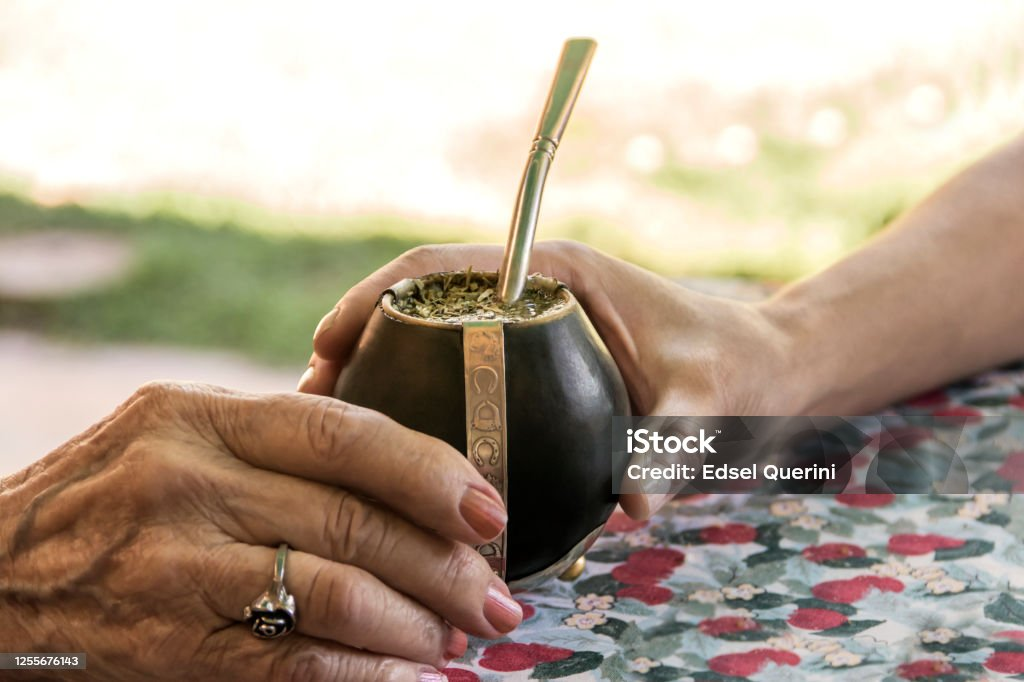
\includegraphics[width=\textwidth]{./media/imagen1.jpg}
%\caption{Este es el epígrafe de la figura a color, véase \textcite{@3159-FUNES2006}.}
%\end{figure}
%\else
%	\ifBLACKPDF%
%	\begin{figure}[!ht]
%	\centering
%	
\includegraphics[width=\textwidth]{./media/bn-imagen1.png}
%	\caption{Este es el epígrafe de la figura en escala de grises.}
%	\end{figure}
%	\else
%		\ifODT%
%		\begin{figure}[!ht]
%		\centering
%		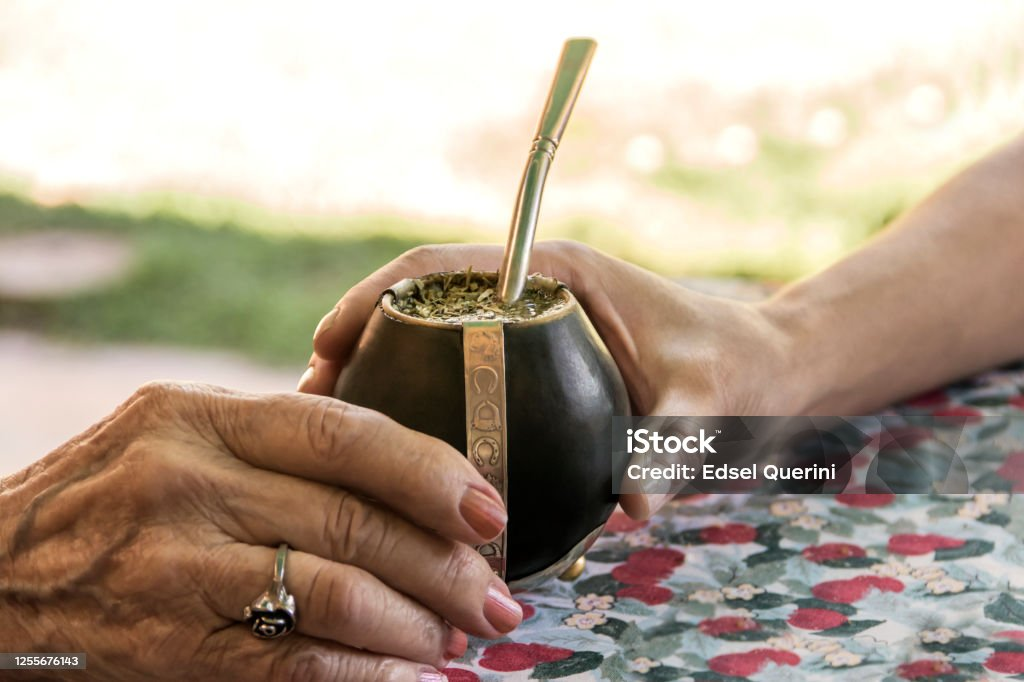
\includegraphics[width=\textwidth]{./media/imagen1.jpg}
%		\caption{Este es el epígrafe de la figura a color.}
%		\end{figure}
%		\else
%			\ifEPUB
%			\begin{figure}[!ht]
%			\centering
%			
\includegraphics[width=\textwidth]{./media/bn-imagen1.png}
%			\caption{Este es el epígrafe de la figura a color.}
%			\end{figure}
%			\fi
%		\fi
%	\fi
%\fi
%
%\section{SecciónBB}
%
%Esta obra colectiva da continuidad a uno de los programas centrales impulsados por el \gls{@glo201-ceheal} desde su creación en 2019: el estudio de las ideas y del pensamiento económico en su vínculo con la implementación de políticas económicas.\footnote{Nota a pie en una sección del segundo capítulo.}

\backmatter

\ifPDF
\printnoidxglossary[type=\acronymtype,title={Índice de siglas}]
\printnoidxglossary[title={Glosario de términos}]
\printbibliography[heading=none,heading=bibintoc]
\printindex[names]
\printindex[concepto]
\printindex[onomastico]
\Author{Índice de autoras y autores}
	\else
	\ifBLACKPDF
		\printnoidxglossary[type=\acronymtype,title={Índice de siglas}]
		\printnoidxglossary[title={Glosario de términos}]
		\printbibliography[heading=none,heading=bibintoc]
	\printindex[names]
	\printindex[concepto]
	\printindex[onomastico]
	\Author{Índice de autoras y autores}
		\else
	 	\ifEPUB
	 	\begingroup
	 	\parindent 0pt
	 	\parskip 2ex
	 	\def\enotesize{\normalsize}
	 	\theendnotes
	 	\endgroup
	 	\printnoidxglossary[type=\acronymtype,title={Índice de siglas}]
	 	\printnoidxglossary[title={Glosario de términos}]
	 	\chapter{Referencias bibliográficas}
	 	\printbibliography[heading=none]
	 	\printindex[names]
	 	\printindex[concepto]
	 	\printindex[onomastico]
	 		\else
	 		\ifHTML
	 		\ForceHTMLPage
	 		\printnoidxglossary[title={Índice de siglas},type=\acronymtype]
	 		\ForceHTMLPage
	 		\printnoidxglossary[title={Glosario de términos}]
	 		\ForceHTMLPage
	 		\printbibliography[heading=bibintoc]
	 			\else
	 			\ifODT
	 			\printnoidxglossary[type=\acronymtype,title={Índice de siglas}]
	 			\printnoidxglossary[title={Glosario de términos}]
	 			\printbibliography[heading=none,heading=bibintoc]
	 			\fi
	 		\fi
		\fi
	\fi
\fi



\chapter{Colofón}

La composición tipográfica de este libro se realizó utilizando \href{https://github.com/albertomoyano/gbtexpublisher}{gbTeXpublisher.}

Las familias tipográficas utilizadas dentro del libro son: IBM Plex, una superfamilia de tipografía abierta, diseñada y desarrollada conceptualmente por Mike Abbink en IBM con colaboración de Bold Monday y Libertinus, bifurcación de la fuente Linux Libertine, diseñada para el texto del cuerpo y la lectura extendida.

\ifPDF
\newpage
\thispagestyle{empty}
{\textcolor{white}{.}}
	\else
	\ifBLACKPDF
	\newpage
	\thispagestyle{empty}
	{\textcolor{white}{.}}
	\fi
\fi

\end{document}



